\documentclass[DM,lsstdraft,toc]{lsstdoc}
\usepackage{graphicx}
\usepackage{url}
\usepackage{latexsym}
\usepackage{color}
% black, blue, brown, cyan, darkgray, gray, green, lightgray, lime, magenta, blue, orange, pink, purple, red, teal, violet, white, yellow.
\usepackage{enumitem}
\usepackage{esvect}

\title[Detection Efficiencies]{Options for Generating Detection Efficiencies for {\tt DIASources}}

\author{M.~L.~Graham et al., and the DM SST}

\setDocRef{DMTN-TBD}
\date{\today}
\setDocUpstreamLocation{\url{https://github.com/lsst-dm/dmtn-tbd}}

\setDocAbstract{ \textcolor{red}{MLG: THIS DOC IS A DRAFT IN PROGRESS. DO NOT CITE.}\\ 
In this study we explore and evaluate options for the generation of detection efficiencies for difference-image point sources detected by Difference Imaging Analysis (DIA).
We review the LSST requirements on characterizing DIA in terms of completeness and purity of detected sources, and compare this with the anticipated needs of the scientific community.
The role of injecting and recovering fake point-sources as a means to generating detection efficiencies is given particular attention.}

\setDocChangeRecord{%
\addtohist{0}{2018-11-01}{Internal working document.}{Melissa Graham}
%\addtohist{2}{yyyy-mm-dd}{Future changes}{Future person}
}

\begin{document}

\maketitle

% CITATION EXAMPLES
% \verb|\citellp|: \citellp{LPM-17, LSE-30} \\
% \verb|\citell|: (SRD; \citell{LPM-17,LSE-29}) \\
% \verb|\citep[][]|: \citep[e.g.,][are interesting]{LPM-17,LSE-29} \\
% \verb|\cite|: \cite{LPM-17,LSE-29}
% \citeds{LSE-163}, \citedsp{LSE-163}


% % % % % % % % % % % % % % % % % % % % % % % % % % % % % % % % % % % %
\section{Introduction} \label{sec:intro}

% This DMTN is associated with JIRA Ticket DM-12584.

A detection efficiency is the probability that a source of a given brightness is detected, given that it exists. In other words, the fraction of all real sources of a given brightness that are detected. This document deals with measuring the detection efficiency for point-sources in a difference image. Difference images are produced by subtracting a template image from a direct image. Template images are not just any other image of the same field: they are generated by stacking previous images in a way that both (1) increases the template's depth and (2) "removes" the flux of transient or moving objects and "standardizes" the flux of variable objects. Point-sources in a difference image are thus the time-changing components of transient and variable objects. The term used by LSST for a source detected via difference imaging analysis is {\tt DIASource}. All scientific analyses that involve population studies or occurrence rates of transient, variable, or moving objects discovered via difference imaging analysis (DIA) require knowing the survey's detection efficiency for point-sources\footnote{We consider the detection efficiencies of extended difference-image sources (e.g., light echoes, trailed moving objects) to be beyond the scope of this study.} in the difference images. Any scientific question which asks, e.g., {\it "How often?"} or {\it "How many?"} about astrophysical phenomena falls into this category of analyses. At all times in this work when we refer generically to a {\it detection efficiency} we mean {\it the detection efficiency of point-sources in difference images}; the detection efficiencies of {\tt DIASources}.

The detection efficiency can be represented as $\eta(m)$, where $m$ is the apparent magnitude of the time-changing component with respect to the template image, and $\eta$ is a value between $0$ and $1$ that represents the probability that the source would be detected in the difference image. In practice, $\eta$ depends on more than just $m$, and can be a function of the parameters ($\vv{P}$) listed in Table \ref{tab:eta_pars}. An accurate measure of $\eta(\vv{P})$ for every pixel of every difference image is technologically unfeasible for most modern imaging surveys, and especially so for the LSST. Instead, it will be necessary to build an analytic model for $\eta$ as a function of the relevant parameters $\vv{P}$ --- some of which may have correlated effects --- which can then be applied to any location in any image. {\bf The topic of this study is the generation of a detection efficiency matrix, $\eta(\vv{P})$, as an LSST data product.}

\begin{table}[h]
\begin{center}
\begin{footnotesize}
\caption[]{A description of the image and source parameters ($\vv{P}$) that can affect the detection efficiency ($\eta$) of point-sources in a difference image (per filter).}
\label{tab:eta_pars}
\setlength{\extrarowheight}{5pt}
\begin{tabular}{|p{3.1cm}|p{12cm}|}
\hline
{\bf Parameter} & {\bf Description} \\
\hline
Apparent Magnitude & Typically, $\eta$ decreases for fainter objects (and brighter objects due to saturation). \\
\hline
Surface Brightness & Typically, $\eta$ decreases for objects embedded in brighter host galaxies. \\
\hline
Static-Source Offset & Sometimes, $\eta$ decreases for objects that are near (i.e., overlap the point-spread function of) static sources (e.g., stars, galaxy cores, especially if cuspy in profile). \\
\hline
CCD Location & With some instruments, $\eta$ decreases near the CCD edges due to distortion. \\
\hline
Image FWHM & The value of $\eta$ can decrease for extreme FWHM differences from the template (i.e., very good or very poor seeing). \\
\hline
Image Airmass & LSST images will experience differential chromatic refraction which affects image subtraction \citedsp{DMTN-037}, and thus potentially also $\eta$. \\
\hline
Sky Brightness & Typically, $\eta$ decreases when the sky background is bright or has a strong gradient (e.g., during twilight, near the moon). \\
\hline
Sky Cloud Cover & Extinction will affect $\eta$ by degrading the image magnitude limit. \\
\hline
\end{tabular}
\end{footnotesize}
\end{center}
\end{table}

\subsection{Study Overview}
\begin{itemize}
\item \S~\ref{sec:sci} contains a primer on the concepts related to detection efficiencies, and an overview of several science goals that rely on them, with examples of methods for generating and applying detection efficiencies from a selection of recent time-domain surveys. 
\item \S~\ref{sec:docs} reviews the LSST Data Management System's (DMS) literature and highlight existing plans, policies, requirements, and specifications related to the generation of LSST survey detection efficiencies. 
\item \S~\ref{sec:opts} presents and evaluates various options for how the DMS could provide detection efficiencies as a data product. 
\item \S~\ref{sec:tech} outlines several techniques for injecting fake point-source variability into images.
\end{itemize}

\subsection{Summary of Study Findings}
\begin{enumerate}
\item It would be most scientifically useful -- with only a small increase in scope -- to ensure that the fake injection of point sources used to characterize the {\tt DIASouce} spuriousness parameter fill the parameter space needed for scientific analyses involving detection efficiencies, and to provide the detection efficiency matrix $\eta(\vv{P})$.
\item It would also be scientifically useful to make catalogs of the injected fakes available to users, to enable them to build detection efficiency matrices, $\eta(\vv{P})$, for their science goals.
\item Further study (simulations) will be needed to identify the optimal mode of fake injection (e.g., modeling the point-spread function or using isolated stars), and the full set of parameters $\vv{P}$ for which $\eta$ should be determined.
\item Soliciting feedback and science use-cases from the community should be considered as a means to prioritize and make decisions regarding the above.
\end{enumerate}

% % % % % % % % % % % % % % % % % % % % % % % % % % % % % % % % % % % %
\section{Scientific Motivation and Use-Cases for Detection Efficiencies}\label{sec:sci}

Section \ref{ssec:sci_rb} introduces the concepts of completeness, purity, and spuriousness for difference-image sources in imaging surveys, and how they are connected to detection efficiency. As described in \S~\ref{sec:docs}, the LSST DMS will characterize {\tt DIASource} completeness and purity as a function of source spuriousness and signal-to-noise ratio (which correlates with source apparent magnitude) --- likely using an analysis of injected fake sources --- but not necessarily as a function of all parameters $\vv{P}$ listed in Table \ref{tab:eta_pars}. Sections \ref{ssec:sci_trans} to \ref{ssec:sci_move} describe how the latter is essential for generating the detection efficiencies for a given population of astronomical objects, and discusses a selection of science use-cases for detection efficiencies in the fields of transients, AGN, variable stars, and moving objects (i.e, similar to science pursued with LSST data). 

% % % % % % % % % % % % % % % % % % % % % % % % % % % % % % % % % % % %
\subsection{Completeness, Purity, and Spuriousness}\label{ssec:sci_rb}

All sources in a survey's difference image are either: \\
\hspace*{10mm} {\bf real} -- caused by a true astrophysical event, or \\
\hspace*{10mm} {\bf bogus} -- an artifact of the telescope hardware or image processing. \\ 
Incompletely removed cosmic rays are considered an artifact, bogus, in this context. 

The {\bf spuriousness} ($\mathcal{S}$) of a source is a value, typically between $0$ and $1$, which represents the probability that a source is real (values closer to $1$) or bogus (values closer to $0$). The spuriousness is sometimes also called the {\it real/bogus score}, and is often determined by machine learning on many sources that were pre-classified as real or bogus. A {\bf spuriousness threshold} ($\tau_{\mathcal{S}}$) is applied to classify the sources deemed likely to be real as {\it detected} by the survey. By raising and lowering the value of $\tau_{\mathcal{S}}$ between $1$ and $0$, the set of detections can be made either more pure (higher $\tau_{\mathcal{S}}$) or more complete (lower $\tau_{\mathcal{S}}$). 

The following definitions categorize the possible states of all real (astrophysical) and bogus (artifact) sources, where "positive" means "detected" and "negative" means "not detected": \\
\hspace*{10mm} {\bf True Positive} ($\mathit{TP}$) -- an astrophysical source that was detected. \\
\hspace*{10mm} {\bf False Positive} ($\mathit{FP}$) -- an artifact that was detected. \\
\hspace*{10mm} {\bf True Negative} ($\mathit{TN}$) -- an artifact that was not detected. \\
\hspace*{10mm} {\bf False Negative} ($\mathit{FN}$) -- an astrophysical source that was not detected. 

The survey's {\bf completeness} ($\mathcal{C}$) is the fraction of all real sources that are detected, which we will here call the true positive rate, $\mathit{TPR} = \frac{\mathit{TP}}{\mathit{TP}+\mathit{FN}}$. The $\mathit{TPR}$ is equivalent to the detection efficiency, $\eta$, which was introduced in Section \ref{sec:intro}. The missed detection rate is the fraction of all real sources that were not detected, $\mathit{MDR} = 1 - \mathit{TPR} = \frac{\mathit{FN}}{\mathit{TP}+\mathit{FN}}$. 

The survey's {\bf purity} ($\mathcal{P}$) is the fraction of all detections that are real astrophysical sources, $\frac{\mathit{TP}}{\mathit{TP}+\mathit{FP}}$. This is also called the {\it precision} or the {\it positive predictive value} ($\mathit{PPV}$) of the survey. The false positive rate\footnote{Note that in some cases the false positive rate is defined as the fraction of all artifacts that are detected, $\mathit{FPR} = \frac{\mathit{FP}}{\mathit{TN}+\mathit{FP}}$, and not the fraction of all detections that are artifacts, $\frac{\mathit{FP}}{\mathit{TP}+\mathit{FP}}$, as we have used here.} is then $\mathit{FPR} = 1 - \mathit{PPV} = \frac{\mathit{FP}}{\mathit{TP}+\mathit{FP}}$. 

\begin{figure}
\begin{center}
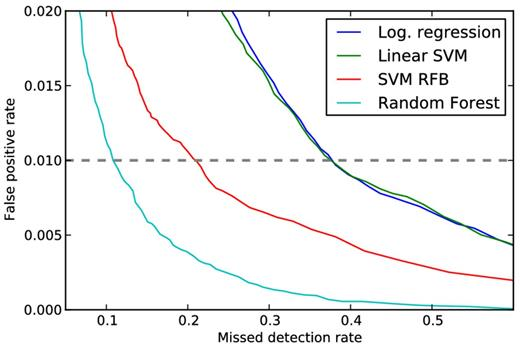
\includegraphics[width=8cm,trim={0cm 0cm 0cm 0cm}, clip]{figures/Brink_etal_2013_Fig3.jpg}
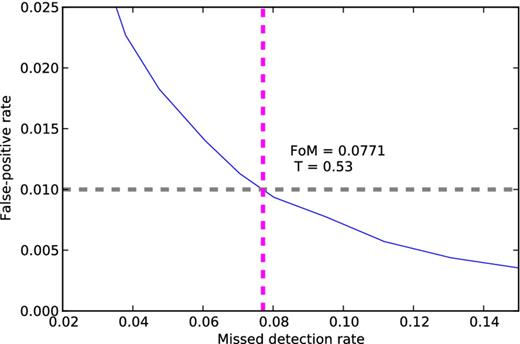
\includegraphics[width=8cm,trim={0cm 0cm 0cm 0cm}, clip]{figures/Brink_etal_2013_Fig7.jpg}
\caption{{\it Left:} An example of the relationship between the false positive rate ($\mathit{FPR}$; purity) {\it vs.} the missed detection rate ($\mathit{MDR}$; completeness) for different types of source classification algorithms considered by the Palomar Transient Factory \citep{2013MNRAS.435.1047B}. {\it Right:} The relationship between $\mathit{FPR}$ and $\mathit{MDR}$ for the RB2 (real-bogus version 2) classifier (blue line) developed by the PTF and introduced in \cite{2013MNRAS.435.1047B}. Dashed lines show how $\mathit{FPR}=0.01$ is achieved with a spuriousness (real-bogus score value) threshold of $\tau=0.53$, which results in $\mathit{MDR}=0.077$. \label{fig:comp_pure}}
\end{center}
\end{figure}

The relationship between the completeness and purity of a sample of {\it detections} can be traced out by varying $\tau_{\mathcal{S}}$. In Figure \ref{fig:comp_pure} we show an example of the relationship between the false positive rate ($\mathit{FPR}$; purity) {\it vs.} the missed detection rate ($\mathit{MDR}$; completeness) for different types of source classification algorithms from the Palomar Transient Factory \citep[PTF;][]{2013MNRAS.435.1047B}. This relationship is formally known as the Receiver Operating Characteristic (ROC) curve when it is plotted as the true positive rate {\it vs.} the false positive rate. 

Characterizing the completeness and purity of a survey requires knowing, {\em a priori}, which of the detected sources are truly real ($\mathit{TP}$), and how many real sources there are in total ($\mathit{TP}+\mathit{FN}$). This is only possible in two scenarios: (1) if co-temporal imaging data of superior quality is in hand (i.e., ``truth" images), or (2) if sources have been simulated and added to the data. However, co-temporal imaging data of superior quality almost never exists (because it is inefficient to duplicate data). Typically, the simulation and injection of fake sources are used to generate a sample of ``real" sources, so that the completeness ($\mathcal{C}$, $\mathit{TPR}$, $\mathit{MDR}$) and purity ($\mathcal{P}$, $\mathit{PPV}$, $\mathit{FPR}$) of the survey and its data processing pipelines can be characterized. 

In order to identify a set of {\it detections} with the completeness and purity required for a given scientific analysis, surveys use the characterized relationship between $\mathcal{C}$, $\mathcal{P}$, and $\mathcal{S}$ to define and impose a spuriousness threshold $\tau_{\mathcal{S}}$ on the full sample. The LSST will derive these quantities and provide them to users (\S~\ref{sec:docs}), but only as a function of source signal-to-noise ratio (or apparent magnitude), and not necessarily as a function of the parameters $\vv{P}$ listed in Table \ref{tab:eta_pars}.

% % % % % % % % % % % % % % % % % % % % % % % % % % % % % % % % % % % %
\subsection{Transients}\label{ssec:sci_trans}

Transient events such as stellar explosions (supernovae, kilonovae) and tidal disruption events (stars destroyed by close passage to a supermassive black hole) occur once and do not repeat. Since most transient progenitors are stars, they are most often found in high surface brightness environments (i.e., galaxies; their spatial distribution ``follows the light") and require difference imaging in order to be discovered, and thus detection efficiencies in order to characterize their occurrence rates. For example, transient occurrence rates as a function of environment can constrain their progenitor star characteristics, which requires that detection biases be well known, as does understanding selection biases in transient samples (e.g., when using Type Ia supernova as cosmological standard candles). 

The following describe four past transient surveys and how they measured their transient detection efficiencies.

{\bf Sloan Digital Sky Survey II (SDSS-II) ---} In order to calculate the occurrence rates of Type Ia supernovae (SNe\,Ia) from the SDSS-II, \cite{2008AJ....135..348S} generated a realistic sample of SNe\,Ia and injected fake point sources into the images as part of the live data processing pipeline to discover SNe\,Ia. Additional simulations to evaluate on how often the fakes were recovered by the end-to-end SN\,Ia discovery pipeline were then required to evaluate how assumptions about the simulated population (e.g., the distribution of light curve stretches) contributed to the final uncertainty in the derived rates \citep{2008ApJ...682..262D}. The final form of their derived detection efficiency for SNe\,Ia was $\epsilon(z) = (0.78 \pm 0.01) + (-0.13 \pm 0.14)z$, within which is captured assumptions about the true relative fraction of each SN\,Ia subtype, such as the under/over-luminous 91bg/91T-likes \citep{2008ApJ...682..262D}. The detection efficiency, $\epsilon$, contributed to the final volumetric rate, $r_V = N / \widetilde{VT\epsilon}$, where $N$ is the number of SNe\,Ia detected, and $\widetilde{VT\epsilon}$ is the product of the effective survey volume, time, and detection efficiency.

{\bf Dark Energy Survey (DES) ---} In order to determine the SN\,Ia detection efficiency as a function of redshift, the DES team used a method very similar to SDSS-II: fake sources were injected into their live data, which was run through their real-time {\tt DiffImg} pipeline used to detect transients \cite{2015AJ....150..172K}. This process also started by simulating a realistic sample of SNe\,Ia, with parameters such as light curve stretch, host offset, and subtype drawn from established underlying distributions, and then used a Monte Carlo simulation of many more SN light curves, combined with the detection efficiencies for their fakes, to determine the SN\,Ia detection efficiency as a function of redshift.
% The DES real/bogus algorithm an pipeline are described by Goldstein et al. 2015:
% http://adsabs.harvard.edu/abs/2015AJ....150...82G

{\bf A Canada-France-Hawaii Telescope (CFHT) Cluster Survey ---} In order to calculate the occurrence rate of SNe\,Ia in galaxy clusters for a CFHT imaging survey, \cite{2012ApJ...746..163S} performed DIA to detect SNe in real time, but the fake injection was done separately. Simulated point sources were implanted into a representative subset of their images, and detection efficiencies calculated as a function of the relevant parameters for this survey: apparent magnitude, image quality, and focal plane location (because because the survey used single pointings with only small dithers). Their expression for the rate of Type Ia supernovae per unit stellar mass is $R_{\rm Ia} = (N_{\rm Ia} / C_{\rm spec}) / ( \sum_{j=1}^{j=N_{\rm img}} \Delta t_j Mj )$, where $N_{\rm Ia}$ is the number of SNe\,Ia discovered in the survey, $C_{\rm spec}$ is the spectroscopic confirmation rate (determined separately), the denominator's sum is over all images of the survey, $M_j$ is the total stellar mass within the image, and $\Delta t_j$ is the control time for SNe\,Ia of that image. The control time is expressed as $\Delta t = \int_{t_1}^{t_2} \eta(m(t)) dt$, where $m(t)$ is a SN\,Ia light curve, $\eta$ is the detection efficiency, and the integration limits are the survey's temporal boundaries. The Monte Carlo method was then used to calculate $R_{\rm Ia}$ for the survey many times while sampling over a realistic distribution of SN\,Ia light curve properties for $m(t)$ and the errors in $N_{\rm Ia}$, $M_j$, and $eta$. During this MC, an {\it effective} detection efficiency was used, which accounts for the possibility that the simulated SN\,Ia was detected in the previous two images: $\eta = \eta_j - \eta_j \eta_{(j-1)} - \eta_j \eta_{(j-2)} - \eta_j \eta_{(j-1)} \eta_{(j-2)}$ (as was appropriate for this surveys monthly cadence). The final result was quoted as the median of the MC rates with $1\sigma$ errors. A similar methodology was applied to this survey's cluster SNe\,II in \cite{2012ApJ...753...68G}.

%%% MLG: old (longer) way to say the above.
% Compared to SDSS-II and DES, a slightly different approach to the SN\,Ia rate calculation is taken by \cite{2012ApJ...746..163S} for a survey which is based on monthly imaging with the MegaCam 1 square degree imager on CFHT. Although SN detections were made in real-time, the fake injection was not done promptly. Instead, fakes were implanted into a representative subset of their images, and detection efficiencies (in this case, represented by $\eta$) were calculated as a function of the relevant parameters for this survey: apparent magnitude, image quality, host offset, and location in the focal plane. 
% As presented in \cite{2012ApJ...746..163S}, the rate of Type Ia supernovae, $R_{\rm Ia}$, per unit stellar mass $\rm SNe\, M_{\odot}^{-1}$, is given by $R_{\rm Ia} = (N_{\rm Ia} / C_{\rm spec}) / ( \sum_{j=1}^{j=N_{\rm img}} \Delta t_j Mj )$, where $N_{\rm Ia}$ is the number of SNe\,Ia discovered in the survey and $C_{\rm spec}$ is the fraction of discovered SNe that were spectroscopically confirmed (determined separately). In the denominator, the sum is over all images of the survey, where $M_j$ is the total stellar mass within the image and $\Delta t_j$ is the control time of that image: $\Delta t = \int_{t_1}^{t_2} \eta(m(t)) dt$, where $m(t)$ is a SN's light curve (apparent magnitude, $m$, as a function of time, $t$), $\eta$ is the detection efficiency for image $j$, and the integration limits are the survey's temporal boundaries. 
% The control time of a given image for a given SN light curve must also account for the probability that the light curve was detected in a prior image. For this particular CFHT program -- a $\sim$monthly survey of SNe\,Ia at low-redshift -- at most the two previous images need be considered. Therefore the detection efficiency $\eta$ used in the above equation was: $\eta = \eta_j - \eta_j \eta_{(j-1)} - \eta_j \eta_{(j-2)} - \eta_j \eta_{(j-1)} \eta_{(j-2)}$. A realistic sample of simulated SN\,Ia light curves, $m(t)$, is then used to calculate a set of $R_{\rm Ia}$, and the median and $1\sigma$ errors are quoted as the final derived SN\,Ia rates per unit stellar mass. Once the detection efficiencies, $\eta$, are calculated, they can be applied to {\it any simulated set of light curves} for which an event rate is desired; for example, see the rates of Type II supernovae (SNe\,II) presented for the same survey in \cite{2012ApJ...753...68G}.

% Frohmaier uses stars from the field, not a simulated PSF: "clone-stamping".
% Frohmaier 2019 details: r_v(z) = (1/V deltaT) sum_{i=1}^N (1+z_i) / epsilon_i
% r_v(z) = volumetric rate of SNeIa at redshift z
% V = volume
% delta T = survey time
% sum over the number of SNeIa in the final sample
% (1+z_i) = cosmological time dilation factor
% epsilon_i = "detection efficiencies of each object"
% but note that epsilon != eta, rather epsilon is built from eta
% a large sample of SNeIa with realistic intrinsic properties are simulated, planted in the data, and then recovered, and then a grid of recovery fractions as a function of SNIa intrinsic properties and redshift is created, and those are the epsilons assigned to detected SNeIa
{\bf Palomar Transient Factory (PTF) ---} The PTF covered $8000$ square degrees with a three-to-five day cadence and generated over $1$ $\rm PB$ of data. As detailed by \cite{2017ApJS..230....4F}, inserting fake sources into all of these images was both impractical and unnecessary. Instead, they chose a single representative {\it field} and planted fake sources in all images of that field. The fakes were given a uniform distribution in apparent magnitude, distributed in each image such that most of them are located within a galaxy, and then the PTF detection efficiencies were determined as a function of the apparent magnitude, the local surface brightness, and image parameters such as FWHM, airmass, moon illumination fraction, and sky background. These detection efficiencies were used to derive the volumetric rate of normal SNe\,Ia \citep{2019MNRAS.tmp..772F}, of Ca-rich transients by \cite{2018ApJ...858...50F}, and of tidal disruption events\footnote{However, note that some rates analyses for TDEs have used aperture photometry and not difference imaging, and thus did not need fake injection for difference-image detection efficiencies (e.g., \cite{2016MNRAS.455.2918H}); see also the treatment of AGN in \S~\ref{ssec:sci_agn}.} (TDEs) by \cite{2018ApJS..238...15H}.

{\bf Transients Summary --} The four surveys mentioned here as examples have either inserted fakes into all of their live images (SDSS-II and DES) or into a representative set of images at a later time (CFHT and PTF), to ensure that detection efficiencies can be determined for the full range of image parameters. In all cases, the fakes were simulated with parameter distributions (e.g., brightness, location) that roughly mimic the real astrophysical objects of interest for each particular survey (mostly supernovae, for the above examples). Typically, the MC method was then used to simulate light curves for the transient of interest, and then the derived detection efficiencies were applied. The take-away message is that, for LSST to best serve a broad section of the transient community, the simulated population of fake sources need only be representative of true astrophysical sources in a bulk sense, in terms of their brightness and location (i.e., plant more faint sources than bright, and more in high surface-brightness areas than isolated regions). The simulated fakes do not need to accurately represent astrophysical transient types, colors, redshifts, durations, light curves, etc., or be planted in sequential images in a correlated way to represent real light curves. That aspect of the analysis is best left to the user to handle during the MC simulation stage for their particular transient type. 

% % % % % % % % % % % % % % % % % % % % % % % % % % % % % % % % % % % %
\subsection{Active Galactic Nuclei}\label{ssec:sci_agn}

Active Galactic Nuclei (AGN) are powered by a supermassive black hole in the center of a galaxy, surrounded by a gas disk. Their energy output is non-thermal emission from X-ray through to mid-infrared, including emission lines in the optical spectrum, and many (or most) AGN exhibit optical variability. As such, they appear as a variable point source in the cores of galaxies. Many studies of AGN use aperture photometry on direct images, and not difference imaging, because it is desirable to have the {\it entire} flux of the AGN's point-source, not just the flux in its variable component. Both AGN and TDE occur in galaxy cores, but since TDE studies typically desire the flux from the event only -- with any underlying point source from the galaxy nucleus removed -- difference imaging is more commonly used for TDE. 

% The first to use variability to select AGN was Sarajedini et al. 2003; an two-epoch HST survey.
AGN samples have typically identified using spectroscopic emission lines, optical colors, or by looking for excesses of radio, X-ray, or mid-infrared emission, but selection by optical variability is also an option and in particular it may be better at including low-luminosity AGN, as described by \cite[e.g.,][]{2008A&A...488...73T,2010ApJ...723..737V}. The detection method of \cite{2008A&A...488...73T} uses image subtraction for the initial detection of AGN candidates, mainly because difference imaging was already done to find supernovae in the survey. Aperture photometry is then performed on the candidates, and a variability threshold applied to form their final sample for spectroscopic follow-up. \cite{2010ApJ...723..737V} skip the difference imaging step and use aperture photometry and a statistical analysis true variability to identify AGN. Neither use the injection of fake point-sources to evaluate their detection efficiencies, and instead use objects with spectra and/or X-ray detections to estimate their completeness. % De Cicco et al. 2015 is very similar to Trevese, done in the VST-SUDARE/VOICE survey for SNe.

However, characterizing the sample selection function for AGN identified by optical variability with spectra or X-ray detections may not be possible in the LSST era, when optical variability will become a more efficient and prolific way to discover AGN \cite[e.g.,][]{2014ApJ...782...37C}, and will be able to generate significantly larger, lower-luminosity, and/or higher-redshift samples for which spectroscopic confirmation is more difficult. With this in mind, a population of fake injected transients to characterize the difference-image detection efficiency of point sources in galaxy cores may be needed by the LSST AGN community. Since SNe also occur in the cores of galaxies \citep[e.g.,][]{2009A&A...507L..17P,2012ApJ...744L..19K}, and quantifying the missed detection rate in the shrouded cores of, e.g., luminous infrared galaxies (LIRGs) remains an open problem, it would be scientifically beneficial to have injected fakes liberally distributed to galaxy cores.

% % % % % % % % % % % % % % % % % % % % % % % % % % % % % % % % % % % %
\subsection{Variable Stars}\label{ssec:sci_varstar}

A star's luminosity might exhibit intrinsic variability (e.g., RR Lyrae, Cepheids) and/or extrinsic variability (e.g., eclipsing binaries, exoplanet transits, or microlensing events). In uncrowded fields, using direct images and the total flux is preferable to difference-imaging analysis for scientific studies that aim to identify and characterize variable stars. However, in crowded fields such as the Galactic plane, identifying variable stars in difference images can be much easier because the difference image is not as (or not at all) crowded, compared to the direct image. For example, the census of variable stars in crowded fields by \cite{2016A&A...588A.128F} describes how difference imaging is used, although it does not appear that injecting fake sources or deriving detection efficiencies was needed for their analysis. It also seems that difference-image detection efficiencies are not needed for microlensing studies, for which it is a common methodology to fit a PSF to every pixel of a difference image, concoct a "light curve", and then statistically assess whether it is consistent with the expected shape of a microlensing event \cite{2015ApJ...806..161L}\footnote{Although \cite{2015ApJ...806..161L} does mention that detection efficiencies would be used in a paper in preparation.}. 

Despite difference-image detection efficiencies not playing a role in past variable star studies, they might still be needed for LSST analyses. For example, injecting new fake sources in crowded stellar fields might be useful for detection efficiencies for stars which are too faint to have a counterpart in the template, but whose variable component makes them detectable by LSST for a short while. This would apply to e.g., M-dwarf flares (a common contaminant in searches for young SNe) and microlensing events. However, simulating variability when there is already a point source in the template image might best be done by means other than fake point-source injection (see \S~\ref{ssec:tech_pre}).

% % % % % % % % % % % % % % % % % % % % % % % % % % % % % % % % % % % %
\subsection{Moving Objects}\label{ssec:sci_move}

All of the moving objects identified by LSST will first be detected as difference-image sources, and detection efficiencies would be useful for population studies. In epochs of non-detection, being able to obtain the detection efficiency at a predicted location (i.e., as a function of local surface brightness and image qualities) would be a useful quantity for science goals related to moving object populations. The probability of, e.g., a faint asteroid's chance alignment over bright galaxies is small, and so fake injected point sources in empty locations may be more useful for moving object science --- these would be needed to simulate very high-redshift transients, as well. A consideration of whether the injection of trailed sources is scientifically useful is left for other work.

% % % % % % % % % % % % % % % % % % % % % % % % % % % % % % % % % % % %
\subsection{Summary of Science Use-Cases}\label{ssec:sci_summary}

The simplest way to serve the time-domain science community is to generate detection efficiencies derived from fake sources injected into images and recovered in the difference images. This population of fake sources should have similar distributions as real astrophysical phenomena in terms of brightness and location (e.g., proximity to static-sky sources, field crowdedness, surface brightness), and the subset of images used should sample the distributions of, e.g., image quality (seeing), sky brightness, and airmass. The simulated fakes do not need to accurately represent astrophysical transient types, colors, redshifts, durations, light curves, etc., or be planted in sequential images in a correlated way to represent real light curves. That aspect of the analysis is best left to the user to handle during the MC simulation stage for their particular type of object. 


% % % % % % % % % % % % % % % % % % % % % % % % % % % % % % % % % % % %
\section{LSST Requirements and Plans Regarding Detection Efficiencies}\label{sec:docs}

Here we review each of the main requirements documents and highlight items that are related to detection efficiencies, and any mentions of fake injection in particular.

The LSST Science Requirements Document \citedsp{LPM-17}) and the LSST System Requirements Document \citedsp{LSE-29} do not make any statements or put any requirements on the detection efficiencies.

% % % % % % % % % % % % % % % % 
\subsection{Observatory System Specifications (OSS)}\label{ssec:docs_oss}

With respect to Prompt data products, the OSS \citedsp{LSE-30} contains several specifications related to the spuriousness parameter in Section 3.1.5.2 ({\it "Level 1 Data Products"}).
\begin{itemize}
\item To develop\ossreq{0351} a metric to characterize the spuriousness of each detected difference image source. There is a specific note that the performance of this metric be assessed {\it "by insertion and recovery of artificial sources"}. (Section 3.1.5.2.1.7.5). 
\item To estimate\ossreq{0352} the completeness and purity as a function of spuriousness threshold for each visit. This will enable users to choose a spuriousness threshold that delivers a sample with the completeness and purity needed for their science goals. (Section 3.1.5.2.1.7.6).
\item To provide\ossreq{0353}\reqparam{transSampleSNR}\reqparam{transCompletenessMin}\reqparam{transPurityMin} a spuriousness threshold that delivers a sample of difference image sources with signal-to-noise ratio $>6$ which is $90\%$ complete and $95\%$ pure (averaged over all visits). (Section 3.1.5.2.1.7.7).
\item To provide\ossreq{0354}\reqparam{orbitObservationThreshold}\reqparam{mopsCompletenessMin}\reqparam{mopsPurityMin} a spuriousness threshold that delivers a sample of difference image sources with signal-to-noise ratio $>5$ which is $>99\%$ complete and $>50\%$ pure (averaged over one month of visits). (Section 3.1.5.2.1.7.8).
\end{itemize}

Although the above specifications require the observatory to provide, for each visit, metrics and thresholds related to the spuriousness parameter as part of the Prompt data products -- and furthermore indicate that fake injection will be part of the derivation of these metrics and thresholds -- these specifications to not require that the fake injection be done as a part of the Prompt processing pipeline. They do indicate, however, that the spuriousness threshold will have to be parameterized in terms of visit image qualities.

With respect to Data Release data products (e.g., direct and coadded images, reprocessed difference images), the OSS specifies\ossreq{0164} that {\it ``object catalog completeness and reliability shall be determined by the data management system"} as a function of magnitude, for objects such as {\it "supernovae at a range of redshifts"}. The OSS furthermore states that provisions be made to enable completeness calculations of other object types {\it "through injection of synthetic objects into the DM pipelines during the Data Release processing (ie. not part of the live data stream)"} (Section 3.1.5.3.2.9, {\it "Level 2 Data Products"}).

{\bf Summary --} The OSS indicates that simulations of fake sources would be used to meet specifications regarding the provision of a spuriousness parameter for difference-image sources, and the thresholds for completeness and purity related to spuriousness, as a function of visit image qualities. 

%%%MLG: This is sufficiently stated in other places.
% For scientific analyses (e.g., Section \ref{sec:sci}), the detection efficiency (completeness) must additionally be known as a function of the source's context, such as local surface brightness (host galaxy background) or proximity to a bright point source (as listed in Table \ref{tab:eta_pars}. The same fake injection routine which meets the OSS's specifications could potentially also be used to derive detection efficiencies in the full parameter space of Table \ref{tab:eta_pars}.


% % % % % % % % % % % % % % % % 
\subsection{Data Management System Requirements (DMSR)}\label{ssec:docs_dmsr}

The DMSR \citedsp{LSE-61} specifies that Data Management System (DMS) shall produce\dmreq{0097} nightly data quality reports that include, among other items, {\it "detection efficiency for point sources vs. mag for each utilized filter"} (it is not specified whether this applies to both direct and difference images). However, based on this requirement's flow-down\footnote{DMS-REQ-0097 is derived from OSS-REQ-0131, {\it ``Nightly Summary Products"}, which describes how the prompt data products shall include nightly reports that summarize the scientific quality of the data and the performance of the observatory and the DMS.}, the intent of this requirement is to provide a nightly summary of the data's bulk scientific quality and the general performance of the observatory and the DMS, not to provide the scientifically useful detection efficiencies that are the topic of this study. 

The DMSR also specifies\dmreq{0009} that the DMS {\it ``shall provide the ability to inject artificial or simulated data into data to assess ... performance"}, and this is derived in part from OSS requirements 0351, 0353, and 0354 discussed in Section \ref{ssec:docs_oss}.

{\bf Summary --} It is clear that the software for fake injection is a deliverable of the DMS, but the DMSR itself does not contain any formal requirements related to using that software to produce detection efficiencies suitable for scientific analyses. 

% As a side note, \citeds{LSE-61} requires that the range of epochs which may contribute to a template image is limited to no more than 1 year\reqparam{templateMaxTimespan}\dmreq{0280}. \citeds{LDM-151} states that TemplateCoadd images should be within a default $2$ years of the current CalExp image which is about to undergo DIA (Section 3.2.3 of \cite{LDM-151}). Taken together, these statements indicate that during DR reprocessing of the DIA data products, there will be as many templates as there are years of survey, and that the multi-year set of {\tt DIASources} for a given {\tt DIAObject} would be generated {\it multiple templates} instead of using just one for a consistent light curve. This is odd.


% % % % % % % % % % % % % % % % 
\subsection{Data Products Definitions Document (DPDD)}\label{ssec:docs_dpdd}

The DPDD \citedsp{LSE-163} does not define a specific data product that represents the difference imaging analysis (DIA) detection efficiencies, but it does include {\tt spuriousness} in the {\tt DIASource} catalog, defining {\tt spuriousness} as {\it ``computed using information from the source and image characterization"}. As discussed in \S~\ref{ssec:docs_oss}, threshold values for {\tt spuriousness} will be provided to generate subsamples of {\tt DIASources} with a given completeness and purity. Recall that {\it spuriousness} represents the probability that a source is astrophysical in origin, given that it was detected -- it cannot be used to derive the probability that an astrophysical source would be detected, given that it exists.

{\bf Summary --} The DPDD does not list any DIA data products that could be used for detection efficiencies or that are directly derived from the fake injection of point sources.

%The {\tt DIASource} catalog table has four parameters that might be scientifically useful for analyses involving detection efficiencies:
%\begin{itemize}
%\item {\tt psLnL [float]} -- {\it Natural log likelihood of the observed data given the point source model.} This represents the probability that a detected source is a point source; detection efficiencies would not apply to non-point sources.
%\item {\tt fpBkgd [float]} $\rm nJy/asec^2$ -- {\it Estimated background at the position (centroid) of the object in the template image.} This will be useful to provide detection efficiencies in difference images as a function of the background at that location.
%\item {\tt fpBkgdErr [float]} $\rm nJy/asec^2$ -- {\it Estimated uncertainty of {\tt fpBkgd}.} Useful in the same way as {\tt fpBkgd}. 
%\item {\tt spuriousness [float]} -- {\it  A measure of spuriousness, computed using information from the source and image characterization, as well as the information on the Telescope and Camera system (e.g., ghost maps, defect maps, etc.).} This is similar to a real/bogus score (\S~\ref{ssec:sci_rb}). As discussed in \S~\ref{ssec:docs_oss}, threshold values for {\tt spuriousness} will be provided to generate subsamples of {\tt DIASources} with a given completeness and purity.
%\end{itemize}

% Regarding the {\tt spuriousness}, the DPDD text further notes that {\it ``The computation of spuriousness will be 'prior free' to the extent possible and not use any information about the astrophysical neighborhood of the source, whether it has been previously observed or not, etc. The intent is to avoid introducing a bias against unusual sources or sources discovered in unusual environments.} The {\tt spuriousness} measure is motivated by OSS-REQ-0351 through 54. In particular, OSS-REQ-0351 states that the spuriousness parameter be assessed by, e.g., {\it ``insertion and recovery of artificial sources"}, and OSS-REQ-0352 states that {\it ``for each visit"}, the completeness and purity of the sample of {\tt DIASources} as a function of a {\tt spuriousness} threshold shall be estimated. 

% Section 3.2 {\it ``Image Characterization Data"} specifies that {\it ``Each processed image .. will record information on the pixel variance ... as well as the per-pixel masks ... These will allow the users to determine the validity and usefulness of each pixel in estimating the flux density recorded in that area of the sky."} But that is more for evaluating uncertainty for analyzes that use pixel fluxes, and not for detection efficiencies in difference images.


% % % % % % % % % % % % % % % % 
\subsection{Data Management Science Pipelines Design}\label{ssec:docs_ldm151}

The Data Management Science Pipelines Design document \citedsp{LDM-151} details the implementation of the requirements set by the SRD, OSS, and DMSR, and how the data products described in the DPDD are generated. \citeds{LDM-151} does not have much to say about detection efficiencies; Section 3, {\it ``Alert Production"}, states that {\it ``In this document we do not address estimation of the selection function for alert generation through the injection of simulated sources. Such a process could be undertaken in batch mode as part of the DRP."} However, \citeds{LDM-151} does make two relevant statements about the {\tt spuriousness} parameter which describe how the real-bogus algorithm will likely {\it ``be based on a trained random forest classifier ... conditioned on the image quality and airmass"} (Section 3.2.4) and that it  {\it ``may use machine learning on other measurements or pixels"} (Section 6.7.2).

{\bf Summary --} \citeds{LDM-151} does not address fake injection -- or any other specific method -- as a means to the {\tt spuriousness} measurements or detection efficiencies.

%Section 3.2.4, {\it ``Difference Imaging"}, states that {\it ``The application of spuriousness algorithms, also known as 'real-bogus', may be applied at this time dependent on whether the number of false positives is less than 50\% of the detected sources. ... The default technique will be based on a trained random forest classifier. It is likely that the training of this classifier will need to be conditioned on the image quality and airmass of the observations."} 

% Section 6.7.2, {\it ``Algorithms"}, states that the {\tt spuriousness} measurement is a {\it ``per-source measure of likelihood the detection is junk (in a difference image)"} that {\it ``may use machine learning on other measurements or pixels"} and {\it ``may be augmented by spuriousness measures that aren't purely per-source"}. Figure 12, a matrix showing the algorithms applied to the different types of measurements (single visit, difference image, etc.) shows that a different implementation or algorithm for {\tt spuriousness} will be used for the Difference Image Measurement compared to the Single Visit, Multi-Coadd, Multi-Epoch, and Forced Measurements.

% Section 5.6.3, {\tt MakeSelectionMaps}, states that this calibration step {\it ``is responsible for producing multi-scale maps that describe LSST's depth and efficiency at detecting different classes of object. The details of what metrics will be mapped, the format and scale of the maps (e.g. hierarchical pixelizations vs. polygons), and the way the metrics will be computed are all unknown".} It also states that this must be extendable to Level 3, but that {\it ``the details of what DM will provide still needs to be clarified to the community"}, and notes that the reprocessing time for fake plants could be prohibitive. However, this referring to the depth and efficiency of detecting static-sky objects in the direct images or deep coadds, not transients/variables in the difference images.

% % % % % % % % % % % % % % % % 
\subsection{Could Detection Efficiencies be Derived from Provided Data Products?}\label{ssec:docs_derDE}

Could the spuriousness parameter $\mathcal{S}$, and the relationship between $\tau_{\mathcal{S}}$ and completeness --- both of which are specified by the OSS to be included in the data products (\S~\ref{ssec:docs_oss}) -- be used to create a full detection efficiency matrix, $\eta(\vv{P})$? In other words, could the following process be used? (1) bin the {\tt DIASources} by $\vv{P}$; (2) calculate the mean spuriousness as a function of apparent magnitude in the bin ($\bar{\mathcal{S}}(m)$); (3) use the established relationship between $\tau_{\mathcal{S}}(m)$ and completeness (\S~\ref{ssec:docs_oss}) to derive $\eta(\vv{P})$.

No. First, the relation between $\tau_{\mathcal{S}}$ and completeness (\S~\ref{ssec:docs_oss}) provides the completeness for all sources with $\mathcal{S}>\tau_{\mathcal{S}}$, whereas the scientific analyses will want the completeness in discrete bins. Second, this relation has already marginalized over parameters $\vv{P}$, and to attempt to "reverse-engineer" them will not be accurate. Third, using the {\tt DIASources} to derive $\eta(\vv{P})$ will lead to a bias, since only {\it already detected} objects are contributing to the detection efficiency. 
% the current OSS requirements are to characterize the relationship between $\tau_{\mathcal{S}}$ and sample completeness {\it only as a function of visit image qualities} (\S~\ref{sec:docs}). 


% % % % % % % % % % % % % % % % 
\subsection{Summary of Existing Requirements and Plans}\label{ssec:docs_sum}

The OSS requires that spuriousness be measured for each detected difference image source, and that spuriousness thresholds are defined and supplied to users in order to create subsets of known completeness and purity for a given signal-to-noise ratio (\S~\ref{ssec:docs_oss}). The OSS furthermore specifies that the spuriousness characterization be done {\it ``by insertion and recovery of artificial sources"}, and that these thresholds are specified to be {\it ``interpreted as an average over the entire survey"} (\S~\ref{ssec:docs_oss}). The DMSR specifies that {\it software} for fake injection is a deliverable of the DMS (\S~\ref{ssec:docs_dmsr}).

There is no requirement or plan regarding the provision of a detection efficiency matrix, $\eta(\vv{P})$, or for the provision of the results of fake injection and recovery from which such a matrix could be built by users. The opportunities for DM to do this are explored in \S~\ref{sec:opts}. As a final note, the DMS computational system is sized to accommodate the (re)processing of all images with fake sources implanted {\bf (get citation for this from K-T)}.




% % % % % % % % % % % % % % % % % % % % % % % % % % % % % % % % % % % %
\section{Options Regarding Detection Efficiencies} \label{sec:opts}

The options for DM to participate in generating detection efficiencies, $\eta(\vv{P})$, are listed and discussed in terms of scope, risk, requirements, and science. 

% % % % % % % % % % % % % % % % 
\subsection{Do Nothing}\label{ssec:opts_no}

In this scenario, the data from any fake injection that is done in order to meet the requirement to characterize the spuriousness is not made available, but the science community would have access to the {\it software} for fake injection.

{\bf Scope --} No expansion of scope. \\
{\bf Risk --} A moderate risk in that multiple user groups may then need to perform fake injection, leading to redundant reprocessing of the data and a computational strain on the resources. \\
{\bf Requirements --} Does not violate or fulfill any requirements. \\
{\bf Science --} This option would negatively impact science results based on transient phenomena, one of the four pillars of LSST science. The need for computationally intensive processing would force multiple teams to compete, and might limit the number of individuals or teams who could successfully derive detection efficiencies, and thus limit the scientific applications.

% % % % % % % % % % % % % % % % 
\subsection{Make Available the Fakes Injected for Spuriousness Characterization}\label{ssec:opts_makefakeavail}

In this scenario, the data generated by the injection and recovery artificial sources in order to meet the requirements to characterize the spuriousness parameter is made available so that users may calculate detection efficiencies. For example, a {\tt DIASource}-like catalog for the fake injected point sources, which users could bin by the $\vv{P}$ relevant to their science and generate $\eta(\vv{P})$. Since the current OSS requirements are to characterize the relationship between $\tau_{\mathcal{S}}$ and sample completeness {\it only as a function of visit image qualities} for {\tt DIASources} with SNR$>$5 (\S~\ref{sec:docs}), this scenario does not guarantee that these artificial sources will be adequate for all science use-cases. 

{\bf Scope --} Possible expansion of scope to make available the fake-source catalogs. \\
{\bf Risk --} Minor risk, if the fake sources do not adequately cover $\vv{P}$, for the same reason as in \S~\ref{ssec:opts_no}. \\
{\bf Requirements --} Does not violate or fulfill any requirements. \\
{\bf Science --} Allowing users to build detection efficiency matrices from the same fake sources as are used to characterize spuriousness would enable at least some scientific analyses.

% % % % % % % % % % % % % % % % 
\subsection{Ensure the Fakes Injected for Spuriousness Characterization Meet Science Goals}\label{ssec:opts_ensurefakeP}

This scenario is similar to that in \S~\ref{ssec:opts_makefakeavail}, except the fake sources that are injected and recovered in order to meet the requirements to characterize the spuriousness parameter are scientifically validated to cover the parameters needed for scientific analyses, $\vv{P}$, as listed in Table \ref{tab:eta_pars}.

{\bf Scope --} Minor expansion of scope to validate the artificial sources cover an adequate range of parameter space, $\vv{P}$, and to make available the fake-source catalogs. \\
{\bf Risk --} No risk. \\
{\bf Requirements --} Does not violate or fulfill any requirements. \\
{\bf Science --} Allowing users to build detection efficiency matrices from a scientifically-validated set of artificial sources would enable more scientific analyses.

% % % % % % % % % % % % % % % % 
\subsection{Generate and Provide Detection Efficiencies}\label{ssec:opts_deteffs}

This scenario takes that of \S~\ref{ssec:opts_ensurefakeP} one step further, and has the DMS generate and provide the detection efficiency matrix, $\eta(\vv{P})$, as a scientifically validated and verified data product.

{\bf Scope --} Moderate expansion of scope to generate $\eta(\vv{P})$. \\
{\bf Risk --} No risk. \\
{\bf Requirements --} Does not violate or fulfill any requirements. \\
{\bf Science --} Enables scientific analyses for all that need detection efficiencies.

% % % % % % % % % % % % % % % % 
%\subsection{Generate Detection Efficiencies Without Fake Injection}\label{ssec:opts_nofakes}
%\textcolor{red}{MLG: I've heard RL say there are other ways to generate detection efficiencies than fake injection, but outside of co-temporal data of superior quality (which will not be available), I'm not sure how to know how many real things are missed as a function of apparent magnitude and other parameters. Maybe RL can fill in this section.}

\subsection{Inject Fakes during Prompt or Data Release Processing?}\label{ssec:opts_fakeswhen}

Here is considered three possible points in the data processing where the fake injection could be performed: during Prompt processing (\S~\ref{sssec:opts_fakeswhen_PP}), on an intermediate timescale between Prompt and Data Release processing (\S~\ref{sssec:opts_fakeswhen_int}), and during DR processing (\S~\ref{sssec:opts_fakeswhen_DR}).

\subsubsection{During Prompt Processing}\label{sssec:opts_fakeswhen_PP}

Inject fake sources into the live data which is processed within 60 seconds of image readout ({\tt OTT1}). With this option, fake sources would be injected {\it on the fly into every new visit image from the telescope processed with DIA} (or into the template image as negatives). This may seem like an extreme option to propose, but as discussed in \S~\ref{ssec:sci_trans} some previous transient surveys have injected fakes into their real-time pipelines, so we consider it here as well. 

{\bf Scientific Motivation for Prompt Fakes --} Surveys that plant artificial sources into live data processing typically use realistic light curves that represent their target population (e.g., color, duration, and location), and inject the fakes into sequential images in order to simulate real transients. The objective of this level of real-time injection is usually not just to characterize the detection efficiency, but also biases in the survey's classification algorithms and/or follow-up programs. Simulating fake sources that represent {\it real transient light-curves} in sequential images and in different filters in a realistic way is {\it not} being proposed here. Furthermore, most of the scientific analyses that require detection efficiencies, such as occurrence rates and population studies, would be done with the DIA products from a data release, and not the prompt products. A continually-updated detection efficiency matrix, $\eta(\vv{P})$, that incorporates data from fakes injected during Prompt processing does not have a strong scientific motivation.

{\bf Interference with Astrophysical Sources -- } In this scenario, fake sources would be planted into new images in a manner that samples the range of parameters for $\eta(\vv{P})$. This process would be comprised of three steps: (1) identify coordinates where the fakes should be planted, (2) fake injection into the image, and (3) bookkeeping for the fakes to ensure they do not contaminate the Alert Stream or the {\tt DIASource} catalog. Fakes should not be injected at random locations because it is important to sample regions with higher surface brightness and to avoid the locations of known {\tt DIAObjects}. If 1000 fakes are  assigned random locations and injected into a 3.2 Gp image, and we assume that image has 10000 (randomly-distributed) true sources in it, then the probability that none of the fakes are coincident with one of the true sources is $0.9968$. However, over a full night of 1000 visits, the probability that none of the fakes ever landed on a true source in any image is $0.0437$, and it is most likely ($P=0.2218$) that 3 fakes would have interfered with true sources. 
% from scipy.stats import hypergeom
% import matplotlib.pyplot as plt
% [M,n,N] = [3200000000,10000,1000]
% rv = hypergeom(M,n,N)
% print( rv.pmf([0,1,2,3,4]) )
% [  9.96843454e-01   3.11521588e-03   4.86216368e-06   5.05362508e-09   3.93505558e-12]
% [M,n,N] = [3200000000000,10000000,1000000]
% rv = hypergeom(M,n,N)
% print( rv.pmf([0,1,2,3,4]) )
% [ 0.04367555  0.13880061  0.21497859  0.22180274  0.17274015]

{\bf Benefits and Drawbacks of Prompt Fakes from a DM Perspective -- } Two of the benefits (to LSST DM) of fake injection during Prompt processing are that (1) it would negate the need for separate re-processing of all fake-infused images, which could increase the total computational budget by up to a factor of $2$, and (2) it could offer real-time feedback on evolution in the survey's completeness or purity, which might be useful --- however, real-time feedback is not a necessary component of the DMS and could be obtained via the spuriousness parameters, as completeness and purity correlate mainly with bulk image properties. Two of the main drawbacks of planting fakes into "live" data are that (1) only a small number should be planted so as to minimize the risk of interference with real phenomena and (2) the additional steps of simulating, planting, and verifying fakes must be included in the computational budget for Prompt processing, which completes within $60$ seconds for every new direct image and is already tightly constrained. 

{\bf Scope --} An expansion of scope in terms of FTE work hours and computational resources. \\
{\bf Risk --} A risk to the DMS by adding three steps to the 60-second processing budget and potentially interfering with the completeness and purity of {\tt DIASources}. \\
{\bf Requirements --} Does not violate any requirements (and is not necessary to meet any requirements). \\
{\bf Science --} This option would provide scientifically useful detection efficiencies, however, it may compromise science results if it interferes with the completeness and purity of {\tt DIASources}. As there would be a limit on the number of fakes injected into every image, and restrictions that those fakes be away from most true transients and variables, this method would not provide the {\it best} characterization of the survey's detection efficiencies.

% % % % % % % % % % % % % % % % 
\subsubsection{On an Intermediate Timescale}\label{sssec:opts_fakeswhen_int}

As a compromise between injecting fakes during Prompt Processing (above) and during Data Release Processing (below), fakes could be injected and recovered on a intermediate timescale (e.g., daily, weekly, monthly). There would be no need to reprocess {\it every} image because the goal is to build up a detection efficiency model as a function of parameters like host background, seeing and airmass. This pipeline could include only images in the parameter space where additional fakes are required. However, as with the proposed option to do fake injection during Prompt processing, there is no science case (or internal use-case) that requires the detection efficiencies updated in real time.  

{\bf Scope --} An expansion of scope in terms of both FTE and computational resources of the DMS. \\
{\bf Risk --} A risk to the DMS (increasing the amount of processing done in between DRs). \\
{\bf Requirements --} Does not violate any requirements. \\
{\bf Science --} This option would enables rates analyses on the Prompt data products, but these analyses are more likely to be done on the DR data products anyway, so it is unlikely that this option opens the door for any new --- or otherwise inaccessible --- science. 

% % % % % % % % % % % % % % % % 
\subsubsection{During Data Release Processing}\label{sssec:opts_fakeswhen_DR}

The benefits of implanting artificial sources into images during the DIA which occurs as a part of the annual DR processing is that fakes can be injected (1) only in locations where there were no detected {\tt DIASources} and (2) in all images without increasing the total computational budget by any more than is required to inject the PSFs. As described in Section \ref{sec:docs}, it is likely that fake injection would be done as part of DIA during DR processing anyway, in order to characterize the spuriousness parameter. This option is only be adding a step to ensure that the fakes are injected in a way that samples the parameter space $\vv{P}$ (Table \ref{tab:eta_pars}), as needed to use the fakes for detection efficiencies. These DR-derived detection efficiencies could be used on the Prompt data products for the following year. 

{\bf Scope --} A mild expansion of scope in terms of FTE, but potentially not in terms of computational resources. \\
{\bf Risk --} No risks. \\
{\bf Requirements --} Does not violate any requirements. \\
{\bf Science --} Enables science with both the DR and Prompt data products. 

% % % % % % % % % % % % % % % % 
\subsection{Summary of Options}\label{ssec:opts_sum}

It would be scientifically useful -- with only a potential small increase in scope, if any -- to ensure that the artificial sources implanted to characterize the {\tt DIASouce} spuriousness parameter sample the parameter space needed for scientific analyses involving detection efficiencies, $\vv{P}$ (e.g., Table \ref{tab:eta_pars}), and to make the data from the injection and recovery of fake sources available to users so that they can build detection efficiency matrices $\eta(\vv{P})$. It would be even more useful to provide $\eta(\vv{P})$ as a scientifically validated data product. For both scenarios, doing the fake injection during the DIA which occurs as a prt of the annual Data Release processing both achieves the science goals and minimizes scope increase and risk to the DMS.



% % % % % % % % % % % % % % % % % % % % % % % % % % % % % % % % % % % %
\section{Options for Fake Point Source Injection Techniques}\label{sec:tech}

There are a variety of ways in which fake sources can be simulated and injected into the images. Some options are more suitable for transients (\S~\ref{ssec:tech_new}), and some for variable stars (\S~\ref{ssec:tech_pre}). The following is a precursory presentation of the options, some of which have been used in the science studies discussed in \S~\ref{sec:sci}. Typically, artificial sources -- positive or negative -- are added to the direct image {\it before} that image enters the difference imaging pipeline, so that the detection efficiency captures the end-to-end pipeline efficiency for detecting difference-image sources. (This is why fakes are not typically injected into the final difference image prior to source detection).

% % % % % % % % % % % % % % % % 
\subsection{Simulating New Fake Objects}\label{ssec:tech_new}

This applies to point sources that appear where there was no point source in the template image, such as transients like supernovae, variable stars that are undetectable in their quiescent state, and moving objects (assuming they're slow-moving enough to not appear as trailed sources, which is a different problem not included in this study). 

Artificial sources that represent new fake objects would be planted in and around galaxies in a way that samples the environments of known transients (and serves the use-cases of variable stars and moving objects projected on background galaxies), would adequately sample areas of open space where most moving objects, some variable stars, and high-$z$ transients with undetectable hosts will be found, and also in crowded fields where many variable stars will be discovered.

{\bf Model PSF ---} A 2D model for the PSF is added to the direct image in order to simulate a new point source. The shape of the PSF is derived from known trends with, e.g., the focal plane location or airmass (DCR), and the brighter/fatter effect.

{\bf Clone-Stamping ---} A nearby star is cut out and rescaled, and used as the simulated point source. One of the main drawbacks of using clone-stamping with LSST images is that incorporating the brighter/fatter effect into the simulation requires either that a star which is both nearby and of a similar brightness be used or that a model component added to the clone star to appropriately change the shape for the simulated brightness. Another drawback of clone-stamping is that very sparse/crowded fields might not have enough nearby/isolated point sources to use.

To decide between model PSFs and clone-stamping will require some testing in order to properly assess their performance and load on the computational resources. However, since knowing the PSF very accurately is something the LSST DMS will already be doing, it seems likely that the Model PSF option should be easier.

% % % % % % % % % % % % % % % % 
\subsection{Simulating Variability in Real Objects}\label{ssec:tech_pre}

This applies to point sources that appear in both the template and direct image, such as variable stars and AGN. In this case, artificial variability is added to an existing point source in the direct image. Extra steps would need to be taken to ensure any real, low-level variability does not affect the results.

{\bf Model PSF Variable Component ---} A 2D model for the PSF with the desired flux of the variable component of the source is added to the object's 2D profile. This might only be useful for probing small flux changes, as it would be difficult be consistent with the brighter/fatter effect.

{\bf Scaling-in-Place ---} Cutout the star, multiply its 2D profile by a scalar in order to make it brighter or fainter, and add it back to the image. This could be modified to account for the brighter/fatter effect by, e.g., convolving with a kernel that both applies the effect and the desired variability, instead of multiplying by a scalar.

\subsubsection{Planting in a Template Image}\label{ssec:tech_pre_temp}

Could there be situations in which, in order to simulate variability, adding a new point source to the template only, or to both the template and the direct image, is needed? For example, in crowded fields, the detection efficiency for variable components of stars that are faint in the template image might be difficult to accurately measure because faint stars are hard to detect and isolate in crowded fields. This a necessary step in applying either of the two above methods for injecting artificial variability in real objects. Thus, it might be necessary to simulate new faint stars in the template {\it and} the direct image, with some flux difference between them, in order to derive detection efficiencies that are not dominated by the brighter, more well-distinguished stars in a crowded field. This would add complexity to the issue and might further expand the scope of the proposed option to provide scientifically validated injected fakes. 

% % % % % % % % % % % % % % % % 
\section{Summary, Open Questions, and Suggested Future Work}\label{sec:future}

\begin{figure}
\begin{center}
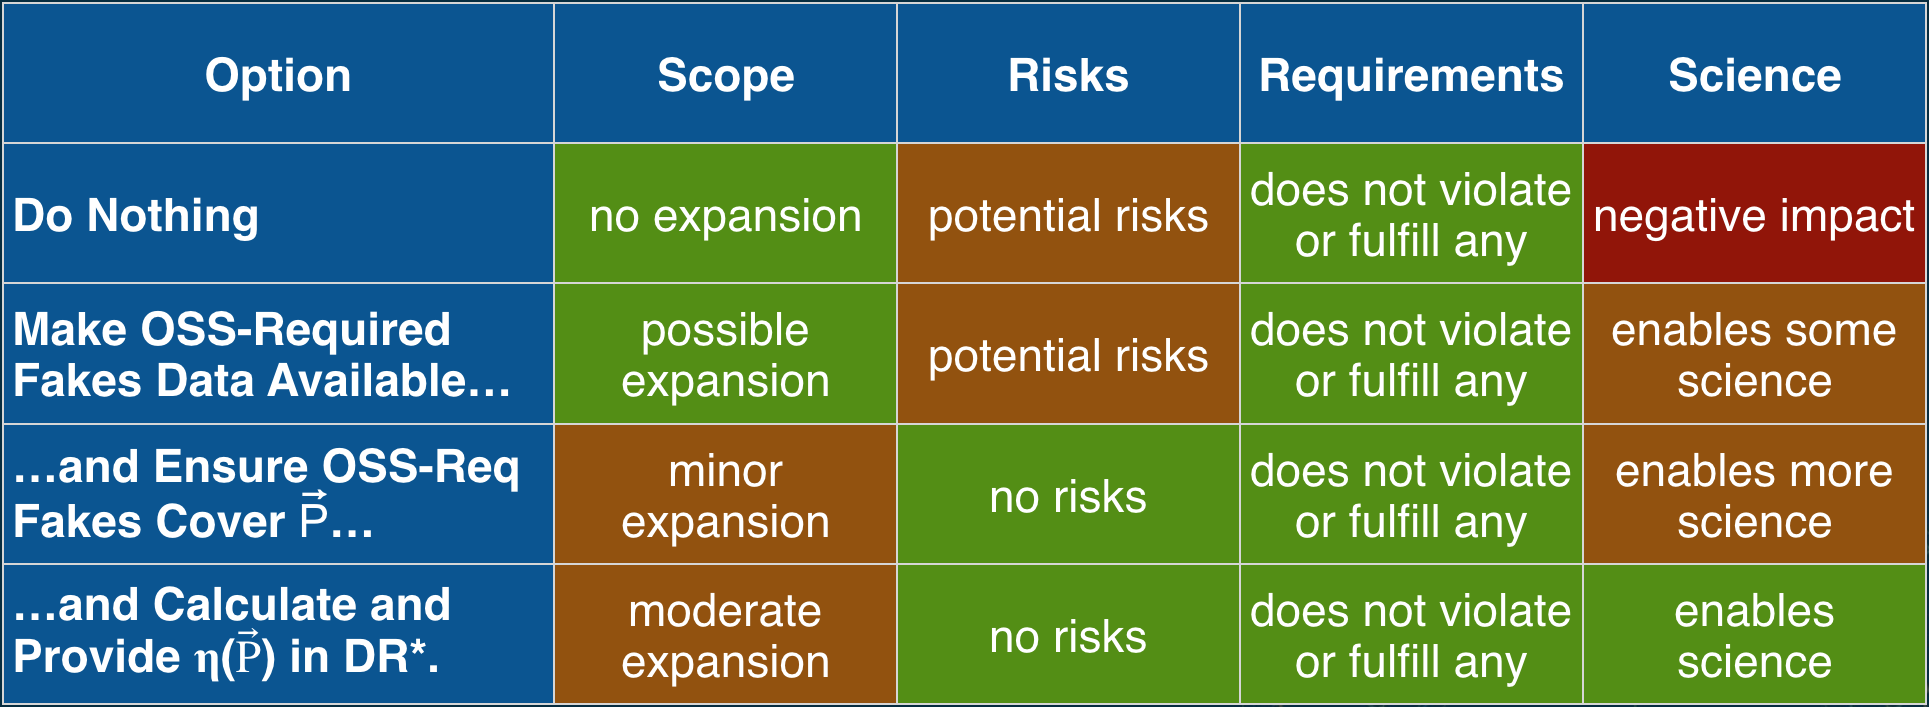
\includegraphics[width=15cm,trim={0cm 0cm 0cm 0cm}, clip]{figures/option_matrix.png}
\caption{A summary of the options with evaluated criteria, based on \S~\ref{sec:opts}. \label{fig:options}}
\end{center}
\end{figure}

This study is not yet finished and there remain some open questions to address, and further work is likely needed in order for an informed decision about the options proposed.

{\bf Open Questions for DM-SST:}\\
(1) Have DM's plans evolved away from what's in the documents (\S~\ref{sec:docs})? \\
(2) Does this work constitute a DMTN? It is not very technical -- yet. One option might be to take this to the TVS community for input and write a joint TVS-DM document, which incorporates the further study items below.

{\bf Further Study:}\\
 - establish the extent of the parameter space, $\vv{P}$\\
 - evaluate the accuracy needed for $\eta(\vv{P})$\\
 - does the mode of fake injection (\S~\ref{sec:opts}) matter for science?\\
 - will LSST's DIA be good enough to simply inject fakes into difference images?\\

% % % % % % % % % % % % % % % % % % % % % % % % % % % % % % % % % % % %
\bibliography{local,lsst,refs,books,refs_ads}
% \appendix
\end{document}


% % % % % % % % % % % % % % % % % % % % % % % % % % % % % % % % % % % %
%%% Sample Table
% \begin{table}[h]
% \begin{center}
% \begin{footnotesize}
% \caption{caption}
% \label{tab:???}
% \begin{tabular}{lll}
% \hline \hline
% C1 & C2 & C3 \\
% \hline
% V1 & V2 & V3 \\
% \hline
% \end{tabular}
% \end{footnotesize}
% \end{center}
% \end{table}
